\input{gitid}

\newcommand{\equ}[1]{eq.~\eqref{equ:#1}}
\newcommand{\Equ}[1]{Eq.~\eqref{equ:#1}}
\newcommand{\fig}[1]{figure~\ref{fig:#1}}
\newcommand{\Fig}[1]{Figure~\ref{fig:#1}}
\newcommand{\sect}[1]{chapter~\ref{sec:#1}}
\newcommand{\Sect}[1]{Chapter~\ref{sec:#1}}
\newcommand{\slink}[2]{\hyperref[#1]{#2}}
\newcommand\votcalogo{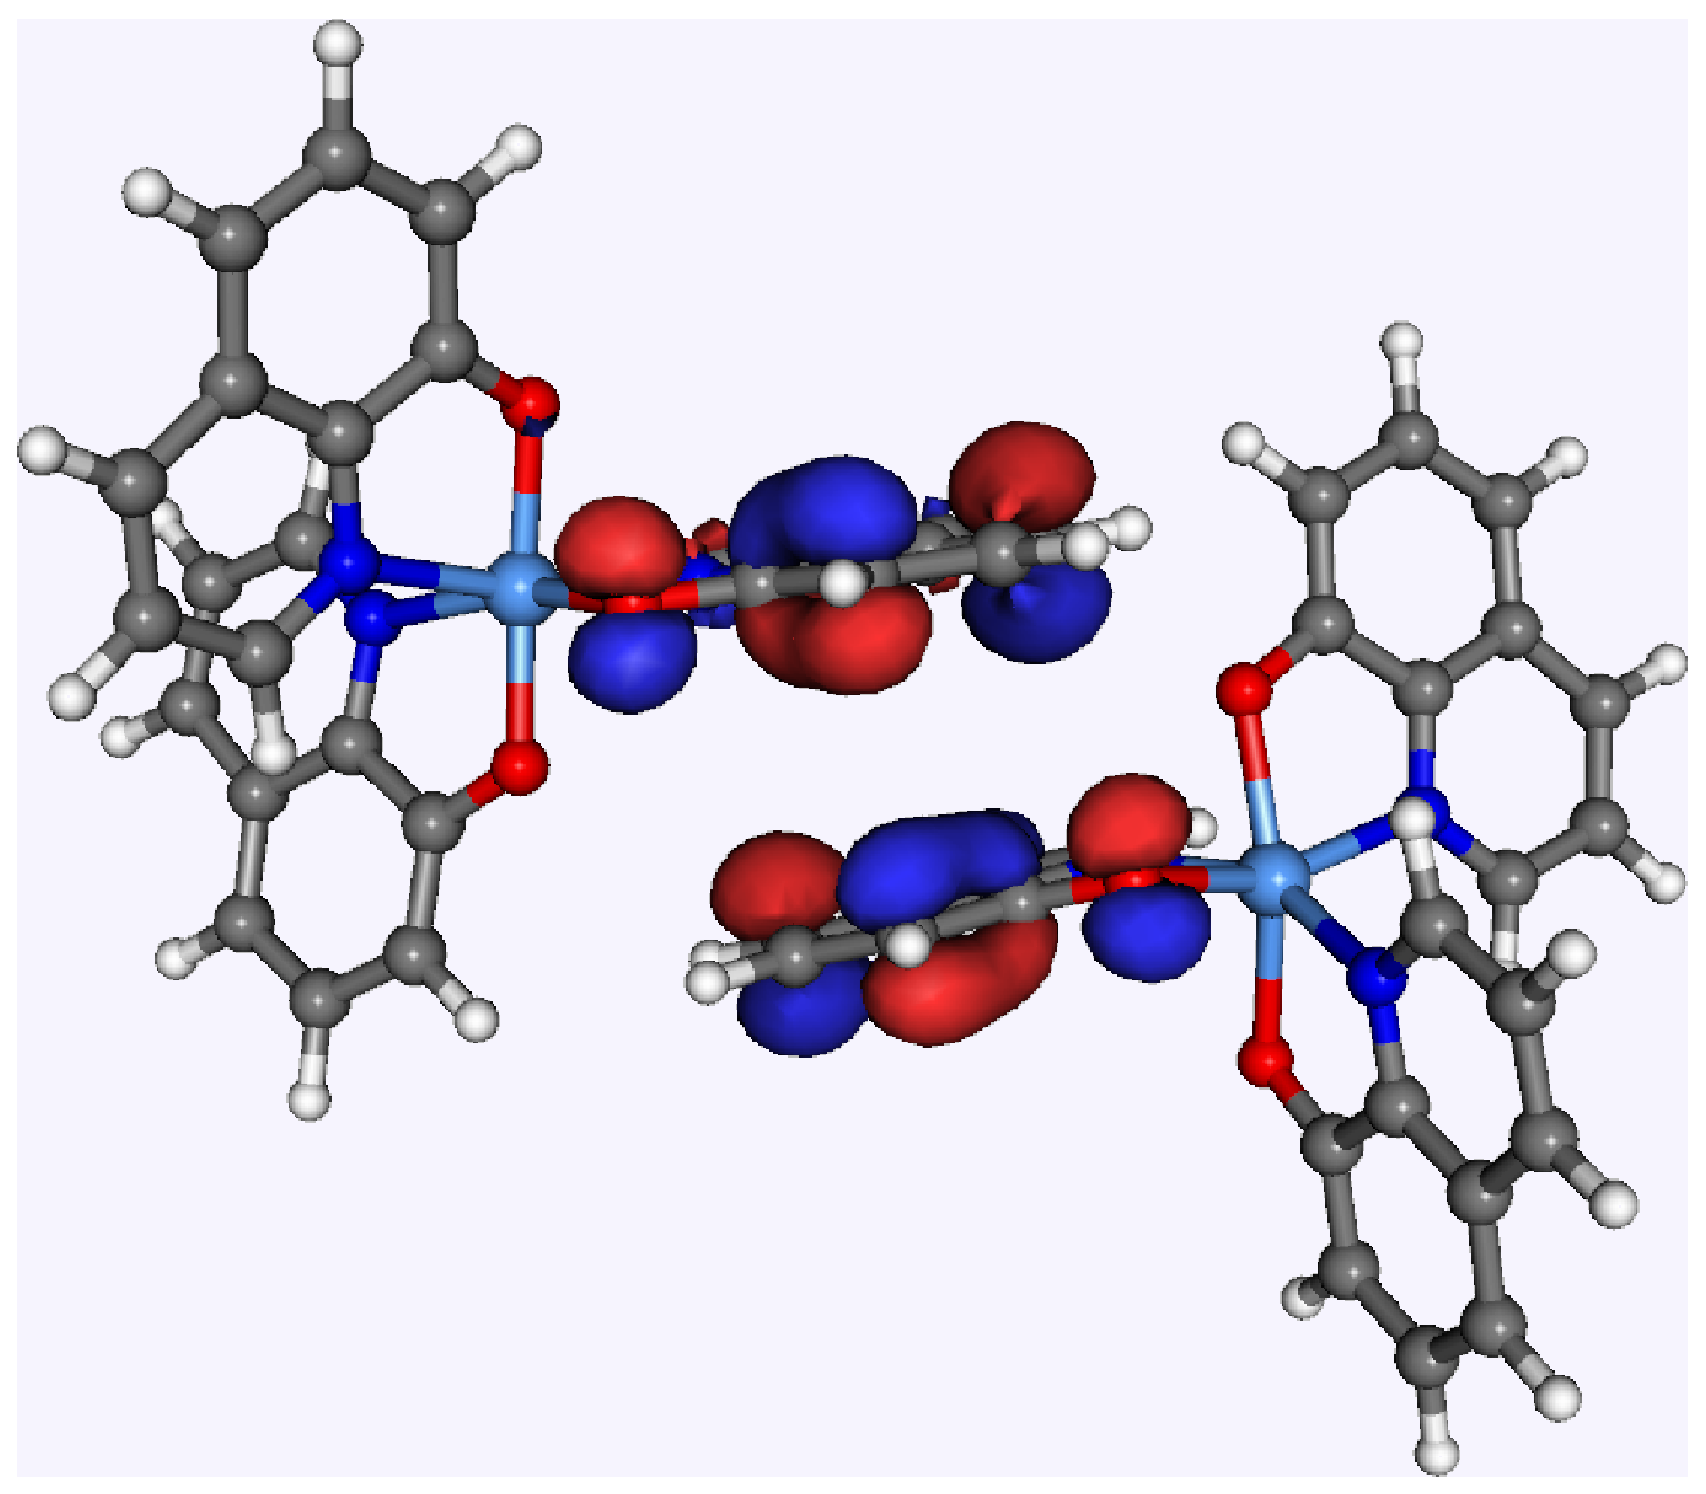
\includegraphics[width=17pt]{fig/logo_trans}}
\newcommand\votcacommand[2]
{
%\begin{bclogo}[couleur=mygray, arrondi =0 , logo=\votcalogo, barre=line,noborder=true]{\small #1}
\itshape {\small #2}
%\end{bclogo}
}

\newcommand\attention[1]
{
%\begin{bclogo}[couleur=mygray, arrondi =0.1 , logo=\bctakecare, barre=line]{\small Be careful!}
{\small #1}
%\end{bclogo}
}

\newcommand{\xml}{XML\xspace}
\newcommand{\gromacs}{\texttt{GROMACS}\xspace}
\newcommand{\gaussian}{\texttt{Gaussian}\xspace}
\newcommand{\turbomole}{\texttt{Turbomole}\xspace}
\newcommand{\nwchem}{\texttt{NWChem}\xspace}
\newcommand{\tinker}{\texttt{TINKER}\xspace}
\newcommand{\dipro}{\texttt{DIPRO}\xspace}

\newcommand{\Alq}{$\mathrm{Alq}_3$\xspace}
\newcommand{\dcvt}{DCV2T\xspace}

\newcommand{\xyz}{\texttt{geometry.xyz}\xspace}
\newcommand{\orb}{\texttt{zindo.orb}\xspace}
\newcommand{\votcaxtp}{{\MakeUppercase{votca-xtp}}\xspace}

\newcommand{\calculator}{\hyperref[sec:calculators]{calculator}\xspace}
\newcommand{\tool}{\hyperref[sec:calculators]{tool}\xspace}

\newcommand{\xmloptions}{\texttt{options.xml}\xspace}
\newcommand{\xmlcsg}{\hyperref[sec:xmlmap]{\texttt{map.xml}}\xspace}
\newcommand{\xmlsegments}{\hyperref[sec:xmlsegments]{\texttt{segments.xml}}\xspace}
\newcommand{\sqlstate}{\hyperref[sec:statefile]{\texttt{state.sql}}\xspace}
\newcommand{\topology}{\texttt{topol.tpr}\xspace}
\newcommand{\trajectory}{\texttt{traj.xtc}\xspace}

\newcommand{\opt}{\texttt{{ -}o}\xspace}
\newcommand{\seg}{\texttt{{ -}s}\xspace}
\newcommand{\sql}{\texttt{{ -}f}\xspace}
\newcommand{\exe}{\texttt{{ -}e}\xspace}
\newcommand{\tpl}{\texttt{{ -}t}\xspace}
\newcommand{\csg}{\texttt{{ -}m}\xspace}
\newcommand{\trj}{\texttt{{ -}c}\xspace}
\newcommand{\job}{\texttt{{ -}j}\xspace}
\newcommand{\run}{\texttt{{run}}\xspace}
\newcommand{\wrt}{\texttt{{write}}\xspace}
\newcommand{\rd}{\texttt{{read}}\xspace}


\newcommand{\refcalc}{\hyperref[ref:calculators]{calculators}\xspace}

\newcommand{\overlap}{\hyperref[prog:xtp_overlap]{\texttt{xtp\_overlap}}\xspace}
\newcommand{\xtprun}{\hyperref[prog:xtp_run]{\texttt{xtp\_run}}\xspace}
\newcommand{\xtpmap}{\hyperref[prog:xtp_map]{\texttt{xtp\_map}}\xspace}
\newcommand{\xtpdipro}{\hyperref[prog:xtp_dipro]{\texttt{xtp\_dipro}}\xspace}
\newcommand{\xtpparallel}{\hyperref[prog:xtp_parallel]{\texttt{xtp\_parallel}}\xspace}
\newcommand{\xtpdump}{\hyperref[prog:xtp_dump]{\texttt{xtp\_dump}}\xspace}
\newcommand{\xtpupdate}{\hyperref[prog:xtp_update]{\texttt{xtp\_update}}\xspace}
\newcommand{\xtptools}{\hyperref[prog:xtp_tools]{\texttt{xtp\_tools}}\xspace}
\newcommand{\kmcrun}{\hyperref[prog:xtp_kmc_run]{\texttt{xtp\_kmc\_run}}\xspace}

\newcommand{\sqlite}{\texttt{sqlite3}\xspace}
\newcommand{\sqlconjsegproperties}{\texttt{conjseg\_properties}\xspace}
\newcommand{\sqlconjsegs}{\texttt{conjsegs}\xspace}
\newcommand{\sqlmolecules}{\texttt{molecules}\xspace}
\newcommand{\sqlpairintegrals}{\texttt{pairintegrals}\xspace}
\newcommand{\sqlpairproperties}{\texttt{pairproperties}\xspace}
\newcommand{\sqlpairs}{\texttt{pairs}\xspace}
\newcommand{\sqlrigidfragproperties}{\texttt{rigidfrag\_properties}\xspace}
\newcommand{\sqlrigidfrags}{\texttt{rigidfrags}\xspace}
\newcommand{\sqlframes}{\texttt{frames}\xspace}


\newcommand{\suggestion}[1]{{\color{red}SUGGESTION: #1}}

\newcommand{\segmentref}[1]{segments.#1}
\newcommand{\segmentopt}[1]{\hyperlink{\segmentref{#1}}{\StrSubstitute{#1}{_}{\_}}\xspace}
\newcommand{\calcref}[1]{#1}
\newcommand{\calcopt}[1]{\hyperlink{\calcref{#1}}{\StrSubstitute{#1}{_}{\_}}\xspace}

\newcommand{\calc}[1]{\hyperref[calc:#1]{\texttt{#1}}\xspace}
\newcommand{\toolref}[1]{\hyperref[tool:#1]{\texttt{#1}}\xspace}

\def\bibsection{%
    \chapter*{Bibliography}%
    \addcontentsline{toc}{chapter}{Bibliography}
}

\renewcommand*{\showkeyslabelformat}[1]{{\normalfont\tiny\sffamily#1}}
\definecolor{refkey}{rgb}{1,0,0}
\definecolor{labelkey}{rgb}{1,0,0}

% Calculus and Linear Algbra Notation
% formulas
\newcommand{\vctr}[1]{\mathbf{ \bar{#1} }}
\newcommand{\oper}[1]{\hat{ #1 }}
\newcommand{\matr}[1]{\mathbf{ #1 }}

%% FULL COMMANDS LISTING
\newcommand{\cmdmap}{\xtpmap \tpl \topology \trj \trajectory \seg \xmlcsg  \sql \sqlstate}
\newcommand{\cmdnbl}{\xtprun \opt \xmloptions  \sql  \sqlstate \exe  \calc{neighborlist}}
\newcommand{\cmdemlt}{\xtprun \opt \xmloptions  \sql  \sqlstate \exe  \calc{emultipole}}
\newcommand{\cmdeint}{\xtprun \opt \xmloptions  \sql  \sqlstate \exe  \calc{einternal}}
\newcommand{\cmdedft}{\xtpparallel \opt \xmloptions \sql \sqlstate \exe \calc{edft}}
\newcommand{\cmdidft}{\xtpparallel \opt \xmloptions \sql \sqlstate \exe \calc{idft}}
\newcommand{\cmdizindo}{\xtprun \opt \xmloptions  \sql  \sqlstate \exe  \calc{izindo}}
\newcommand{\cmdouter}{\xtprun \opt \xmloptions  \sql  \sqlstate \exe  \calc{outersphere}}
\newcommand{\cmdrates}{\xtprun \opt \xmloptions  \sql  \sqlstate \exe  \calc{rates}}
\newcommand{\cmdkmc}{ \kmcrun \opt \xmloptions  \sql  \sqlstate \exe  \calc{kmcmultiple}}
\newcommand{\cmdkmcsin}{ \kmcrun \opt \xmloptions  \sql  \sqlstate \exe  \calc{kmcsingle}}
\newcommand{\cmdeana}{\xtprun \opt \xmloptions  \sql  \sqlstate \exe  \calc{eanalyze}}
\newcommand{\cmdmolpol}{\xtptools \opt \xmloptions \exe \toolref{molpol}}
\newcommand{\cmdlogmps}{\xtptools \opt \xmloptions \exe \toolref{log2mps}}
\newcommand{\cmdxqmult}{\xtpparallel \opt \xmloptions \sql \sqlstate \exe \calc{xqmultipole}}

